\section{Caching}
\label{sec:caching}

In terms of caching, the build pipeline is best evaluated when assuming the best possible, as well as the worst possible case. As already explained in ch. \ref{sec:challenges-cachedetermination} on p. \pageref{sec:challenges-cachedetermination}, such scenarios would be on the one hand a commit only containing content changes (e.g. new or modified blog posts) and on the other hand a commit containing a modification of the default template. Since the default template is very likely to act as a dependency of nearly all content files, a full rebuild is inevitable.

\subsection{Initial build}
An initial build is necessary every time a repository was registered using the REST API, or the repository's previous build attempts constantly failed and no successful outcome was produced yet. Not only caring for the required folder structure, a successful build cycle also provides information for a subsequent rendering process by storing its head commit hash value in the build log on the database. Any following build attempt is able to forge upon the last successful build files.

Therefore it is a good advice to have a successful initial build ready as soon as possible, as future build cycles profit from an early render history and a best possible caching structure. By omitting an early registration to the REST API, any initial build cycle in the future will last a significant amount of time longer, due to continuous progression which is not able to make use of any cached file structure.

%% Graphic of MongoDB entries
\begin{figure} % h-ere, t-op, b-ottom, p-age
    \centering
    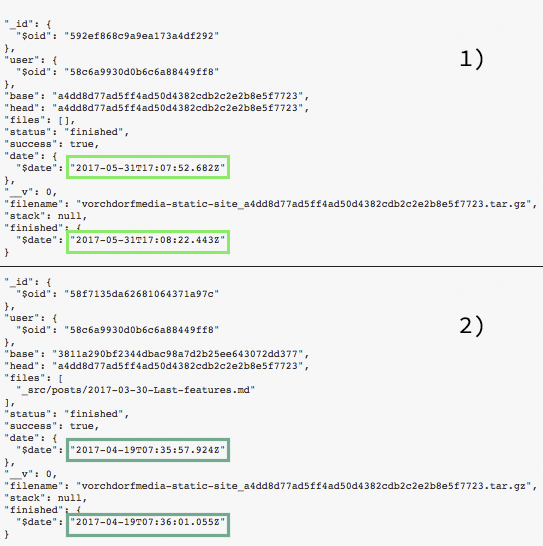
\includegraphics[width=0.9\textwidth]{caching_mongodb.png}
    \caption{Two screenshots of build log entries on the database showing the extent of ideal caching. Example \emph{1)} shows a forced rebuild during the load test (see fig. \ref{fig:pen-test}). Obviously there already happened some successful rendering cycles in the past, as \emph{base} and \emph{head} show the same commit hashes. The build lasted roughly 30 seconds and resulted in a successful archive file.\\
    Example \emph{2)} shows an earlier build, which made use of an available cache. The entry listed in the ``files'' array was the only file, which was rendered and added to the existing file structure. Therefore the build cycle lasted only 4 seconds.}
    \label{fig:caching-mongodb}
\end{figure}
%

\subsection{Caching strategy}
Since caching works most effectively if subsequent commits only contain content changes, the commit culture should be focused towards a content-only development, to make use of a long-lasting series of performant build cycles. Normally, this would be the standard for steady sites containing a significant amount of various information (e.g. FAQ-, support-, or documentation-sites), where constantly changing design decisions are not likely to play an important role. Concerning the need of a templating- or design change, the probably best advice is to collect commits containing such system files for as long as possible before actually merging them into the main branch and causing a longer lasting rebuild task, resulting in a major redesign.

Blogs are also likely to follow this kind of commit pattern, as usually a theme is set once, before subsequent blog posts are published. Using this type of scenario, the extent of ideal caching may be seen on fig. \ref{fig:caching-mongodb}. A rebuild, as well as an initial build at a later time is a lot more time consuming for resulting in a sane file structure, than a selectively rendered build result, which is able to get merged into an existing website root.

Thereby it is not important to check for any existing file structure, if any previously failed build attempt forced a rebuild due to its commit history, as the current build is always able to rely on the rendering result of the last successfully logged attempt.
